\documentclass[11pt]{article}

\usepackage[margin=1in]{geometry}
\usepackage{amsmath,amssymb,amsthm}
\usepackage{booktabs}
\usepackage{enumitem}
\usepackage{graphicx}
\usepackage{hyperref}

% Course notation: vectors bold lowercase, matrices bold uppercase.
\newcommand{\vct}[1]{\mathbf{#1}}
\newcommand{\mat}[1]{\mathbf{#1}}

\graphicspath{{figures/}{hw1/figures/}}
\hypersetup{colorlinks=true,linkcolor=black,urlcolor=blue}

\title{EE 511 Homework 1\\[0.4em]
\large Machine Learning Hardware Accelerators}
\author{Harsha Vardhan}
\date{Fall 2026}

\begin{document}
\maketitle

\paragraph{Notation.}
Vectors are column vectors in \(\mathbb{R}^n\) and are written in bold
lowercase (\(\vct{x}\)); matrices are bold uppercase (\(\mat{A}\)).
\(\mat{A}^\top\) is the transpose, \(\mat{I}_n\) the \(n \times n\) identity,
\(\mathrm{tr}(\cdot)\) the trace, and \(\|\cdot\|_p\) the \(\ell_p\) norm.
``MAC'' means one multiply--accumulate operation (\(=\ 2\) FLOPs).

\tableofcontents
\newpage

\section*{Part A: Theory}
\addcontentsline{toc}{section}{Part A: Theory}

%======================================================================
\section{Problem 1: Inner Products, Norms, and Angular Similarity}
%======================================================================

\subsection*{(a) Cauchy--Schwarz}

I need to prove that for all \(\vct{x}, \vct{y} \in \mathbb{R}^n\),
\[
\bigl|\vct{x}^\top \vct{y}\bigr| \le \|\vct{x}\|_2 \|\vct{y}\|_2.
\]

\paragraph{Equality condition.}
Equality holds if and only if \(\vct{x}\) and \(\vct{y}\) are linearly
dependent: there exists \(\lambda \in \mathbb{R}\) such that
\(\vct{x} = \lambda \vct{y}\). This includes the edge cases
\(\vct{x} = \vct{0}\) and \(\vct{y} = \vct{0}\).

\paragraph{Proof of the inequality.}
Handle \(\vct{y} = \vct{0}\) separately. If \(\vct{y} = \vct{0}\), then
\(\vct{x}^\top \vct{y} = 0\) and \(\|\vct{y}\|_2 = 0\), so both sides are
\(0\) and the inequality holds (as equality). The same argument works if
\(\vct{x} = \vct{0}\).

Now assume \(\vct{y} \neq \vct{0}\). Following the hint, define
\[
g(t) = \|\vct{x} - t\vct{y}\|_2^2 \ge 0 \qquad \text{for all } t \in \mathbb{R}.
\]
Expand:
\begin{align*}
g(t)
&= (\vct{x} - t\vct{y})^\top (\vct{x} - t\vct{y}) \\
&= \vct{x}^\top \vct{x} - t\, \vct{y}^\top \vct{x} - t\, \vct{x}^\top \vct{y}
  + t^2 \vct{y}^\top \vct{y} \\
&= \|\vct{x}\|_2^2 - 2t\,(\vct{x}^\top \vct{y}) + t^2 \|\vct{y}\|_2^2.
\end{align*}
This is a quadratic \(at^2 + bt + c\) in \(t\), with
\[
a = \|\vct{y}\|_2^2 > 0,
\qquad
b = -2\vct{x}^\top \vct{y},
\qquad
c = \|\vct{x}\|_2^2.
\]
Since \(a > 0\) and \(g(t) \ge 0\) for every real \(t\), the parabola never
goes below the axis, so its discriminant satisfies \(\Delta \le 0\):
\[
\Delta = b^2 - 4ac
= 4(\vct{x}^\top \vct{y})^2 - 4\|\vct{y}\|_2^2 \|\vct{x}\|_2^2
\le 0.
\]
Dividing by 4 and taking nonnegative square roots,
\[
(\vct{x}^\top \vct{y})^2 \le \|\vct{x}\|_2^2 \|\vct{y}\|_2^2
\qquad \Rightarrow \qquad
\bigl|\vct{x}^\top \vct{y}\bigr| \le \|\vct{x}\|_2 \|\vct{y}\|_2.
\]

\paragraph{Equality, \(\Rightarrow\).}
Suppose \(\bigl|\vct{x}^\top \vct{y}\bigr| = \|\vct{x}\|_2 \|\vct{y}\|_2\).
If \(\vct{y} = \vct{0}\), then \(\vct{y} = 0 \cdot \vct{x}\), so they are
dependent. If \(\vct{y} \neq \vct{0}\), then \(\Delta = 0\), so \(g\) has a
repeated root \(t_*\). Then \(g(t_*) = 0\), hence
\(\|\vct{x} - t_*\vct{y}\|_2 = 0\), hence \(\vct{x} = t_* \vct{y}\).

\paragraph{Equality, \(\Leftarrow\).}
Suppose there exists \(\lambda \in \mathbb{R}\) with
\(\vct{x} = \lambda \vct{y}\). Then
\[
\bigl|\vct{x}^\top \vct{y}\bigr| = |\lambda| \|\vct{y}\|_2^2,
\qquad
\|\vct{x}\|_2 \|\vct{y}\|_2
= |\lambda| \|\vct{y}\|_2 \cdot \|\vct{y}\|_2
= |\lambda| \|\vct{y}\|_2^2.
\]
The two sides match, so equality holds. (If \(\lambda \ge 0\) they point the
same way and \(\vct{x}^\top \vct{y} = +\|\vct{x}\|_2\|\vct{y}\|_2\); if
\(\lambda < 0\) they point opposite and we get the minus sign. The absolute
value still matches.)

%----------------------------------------------------------------------
\subsection*{(b) Cosine similarity is well defined}

Using part (a), for any nonzero \(\vct{x}, \vct{y} \in \mathbb{R}^n\) we have
\(\|\vct{x}\|_2 \|\vct{y}\|_2 > 0\), so we can divide:
\[
\left| \frac{\vct{x}^\top \vct{y}}{\|\vct{x}\|_2 \|\vct{y}\|_2} \right| \le 1
\qquad \Rightarrow \qquad
\cos\theta
= \frac{\vct{x}^\top \vct{y}}{\|\vct{x}\|_2 \|\vct{y}\|_2}
\in [-1, 1].
\]
That's why the cosine formula is well defined: Cauchy--Schwarz is what keeps
it inside the actual range of cosine.

\paragraph{\(\cos\theta = +1\).}
Take the pair in \(\mathbb{R}^3\)
\[
\vct{x} = \begin{pmatrix} 1 \\ 0 \\ 0 \end{pmatrix},
\qquad
\vct{y} = \begin{pmatrix} 2 \\ 0 \\ 0 \end{pmatrix}.
\]
Then \(\vct{x}^\top \vct{y} = 2\) and
\(\|\vct{x}\|_2 \|\vct{y}\|_2 = 1 \cdot 2 = 2\), so \(\cos\theta = +1\).
Geometrically they are parallel and point in the same direction (angle \(0\)).

\paragraph{\(\cos\theta = -1\).}
Take
\[
\vct{x} = \begin{pmatrix} 1 \\ 0 \\ 0 \end{pmatrix},
\qquad
\vct{y} = \begin{pmatrix} -3 \\ 0 \\ 0 \end{pmatrix}.
\]
Then \(\vct{x}^\top \vct{y} = -3\) and
\(\|\vct{x}\|_2 \|\vct{y}\|_2 = 3\), so \(\cos\theta = -1\).
Geometrically they are parallel but point in opposite directions
(angle \(\pi\)).

%----------------------------------------------------------------------
\subsection*{(c) Norm equivalence}

I need to prove that for any \(\vct{x} \in \mathbb{R}^n\),
\[
\|\vct{x}\|_2 \le \|\vct{x}\|_1
\qquad \text{and} \qquad
\|\vct{x}\|_1 \le \sqrt{n}\, \|\vct{x}\|_2.
\]

\paragraph{First inequality: \(\|\vct{x}\|_2 \le \|\vct{x}\|_1\).}
Compare squares, as in the hint. Expanding
\(\bigl(\sum_i |x_i|\bigr)^2\) gives \(\sum_i x_i^2\) plus nonnegative cross
terms:
\begin{align*}
\|\vct{x}\|_1^2
&= \left( \sum_{i=1}^n |x_i| \right)^2 \\
&= \sum_{i=1}^n x_i^2 + \sum_{i \neq j} |x_i||x_j| \\
&= \|\vct{x}\|_2^2 + \sum_{i \neq j} |x_i||x_j|.
\end{align*}
Each cross term is \(\ge 0\), so \(\|\vct{x}\|_1^2 \ge \|\vct{x}\|_2^2\).
Both norms are \(\ge 0\), so \(\|\vct{x}\|_2 \le \|\vct{x}\|_1\).

Equality when every cross term is \(0\), i.e.\ at most one coordinate is
nonzero. A nonzero vector that attains equality is the sparse standard basis
vector \(\vct{x} = (1, 0, \ldots, 0)^\top\):
\(\|\vct{x}\|_2 = \|\vct{x}\|_1 = 1\). In one sentence: this extremal
\(\vct{x}\) is sparse (1-sparse).

\paragraph{Second inequality: \(\|\vct{x}\|_1 \le \sqrt{n}\,\|\vct{x}\|_2\).}
Apply part (a) to the all-ones vector \(\vct{y} = \vct{1}\) and the
absolute-value vector
\(\vct{z} = (|x_1|, \ldots, |x_n|)^\top\):
\[
\vct{z}^\top \vct{1} = \sum_i |x_i| = \|\vct{x}\|_1,
\qquad
\|\vct{z}\|_2 = \|\vct{x}\|_2,
\qquad
\|\vct{1}\|_2 = \sqrt{n}.
\]
Cauchy--Schwarz gives
\[
\|\vct{x}\|_1
= \bigl|\vct{z}^\top \vct{1}\bigr|
\le \|\vct{z}\|_2 \|\vct{1}\|_2
= \sqrt{n}\, \|\vct{x}\|_2.
\]
Equality when \(\vct{z}\) and \(\vct{1}\) are linearly dependent, i.e.\ all
\(|x_i|\) are equal. A nonzero vector that attains equality is the dense
all-ones vector \(\vct{x} = (1, 1, \ldots, 1)^\top\):
\(\|\vct{x}\|_1 = n\) and \(\sqrt{n}\,\|\vct{x}\|_2 = n\). In one sentence:
this extremal \(\vct{x}\) is dense (equal magnitude in every coordinate).

%----------------------------------------------------------------------
\subsection*{(d) Why accelerators pre-normalize}

A vector database stores \(N = 10^6\) embeddings of dimension \(d = 768\) in
FP32 and must rank all of them against one query \(\vct{q}\). The accelerator
has a 768-lane MAC array, so one full 768-element dot product retires per
cycle. Scalar units are shared and not pipelined: one square root costs 20
cycles, one division costs 30 cycles, and while either is executing the MAC
array stalls. The query's own norm is computed once and cached. Remember
that \(\|\vct{v}\|_2\) for a stored vector is itself a dot product
(\(\vct{v}^\top \vct{v}\)) before it is a square root.

\paragraph{(i) Raw cosine.}
Query norm (cached): \(1\) dot product \(\vct{q}^\top \vct{q}\) and
\(1\) square root.

For each of the \(N\) stored vectors \(\vct{v}_i\):
\begin{itemize}[leftmargin=1.4em]
    \item \(\vct{q}^\top \vct{v}_i\) --- \(1\) dot product
    \item \(\|\vct{v}_i\|_2\) --- \(1\) dot product
         (\(\vct{v}_i^\top \vct{v}_i\)) \(+\) \(1\) square root
    \item \(\dfrac{\vct{q}^\top \vct{v}_i}{\|\vct{q}\|_2 \|\vct{v}_i\|_2}\)
         --- \(1\) division
\end{itemize}
Totals to score the whole database:
\begin{center}
\begin{tabular}{lrr}
    \toprule
    Operation & Symbolic count & Number \\
    \midrule
    Dot products & \(2N + 1\) & \(2{,}000{,}001\) \\
    Square roots & \(N + 1\)  & \(1{,}000{,}001\) \\
    Divisions    & \(N\)      & \(1{,}000{,}000\) \\
    \bottomrule
\end{tabular}
\end{center}

\paragraph{(ii) Pre-normalized to unit \(\ell_2\).}
Every stored vector and the query were normalized to unit \(\ell_2\) length
before ever reaching the accelerator, so
\(\cos\theta = \vct{q}^\top \vct{v}_i\). Scalar units are used zero times.
\begin{center}
\begin{tabular}{lrr}
    \toprule
    Operation & Symbolic count & Number \\
    \midrule
    Dot products & \(N\) & \(1{,}000{,}000\) \\
    Square roots & \(0\) & \(0\) \\
    Divisions    & \(0\) & \(0\) \\
    \bottomrule
\end{tabular}
\end{center}

\paragraph{(iii) Total cycles and end-to-end speedup.}
Raw cosine:
\[
C_{\mathrm{raw}}
= (2N+1)\cdot 1 + (N+1)\cdot 20 + N\cdot 30
= 52N + 21
= 52{,}000{,}021.
\]
Pre-normalized:
\[
C_{\mathrm{pre}} = N \cdot 1 = 1{,}000{,}000.
\]
End-to-end speedup as a ratio of total cycles (not scalar-only, since case
(ii) uses the scalar units zero times):
\[
\frac{C_{\mathrm{raw}}}{C_{\mathrm{pre}}}
= \frac{52{,}000{,}021}{1{,}000{,}000}
= 52.000021
\approx 52\times.
\]
The removed work was not eliminated. It was relocated: each stored vector is
normalized once at ingest (self-dot \(+\) sqrt \(+\) rescale), and the query
is normalized once before it is issued. After that the accelerator only does
the \(N\) dots.

\paragraph{(iv) 1-lane MAC array.}
Now a dot product takes \(768\) cycles.
\[
C_{\mathrm{raw}}
= (2N+1)\cdot 768 + (N+1)\cdot 20 + N\cdot 30
= 1586N + 788
= 1{,}586{,}000{,}788,
\]
\[
C_{\mathrm{pre}} = N \cdot 768 = 768{,}000{,}000,
\]
\[
\text{speedup}
= \frac{1{,}586{,}000{,}788}{768{,}000{,}000}
\approx 2.065\times.
\]
The same optimization looks far less impressive because the dots now dominate
the cycle count, so the 20--30 cycle scalar stalls are a small fraction of
runtime; that tells you scalar-unit latency is worth engineering around only
when the array is already wide enough that a full inner product is cheap.

%----------------------------------------------------------------------
\subsection*{(e) Choosing a norm for the quantizer}

Symmetric INT8 quantization of a tensor \(\vct{x}\) uses
\(s = \|\vct{x}\|_\infty / 127\). After dequant, each entry is \(q_i \cdot s\),
so the representable set is the box \([-127s, 127s]^n\). We avoid clipping
iff \(127s \ge \max_i |x_i| = \|\vct{x}\|_\infty\), and the tightest such
scale is
\[
s = \frac{\|\vct{x}\|_\infty}{127}.
\]
That's why \(\|\vct{x}\|_\infty\) is the correct choice, not
\(\|\vct{x}\|_2\) or \(\|\vct{x}\|_1\). INT8's grid is an axis-aligned box.
\(\ell_2\) is a ball and \(\ell_1\) is a diamond, so neither matches the
codes we actually have. Using \(\|\vct{x}\|_2/127\) would still not clip
(since \(\|\vct{x}\|_2 \ge \|\vct{x}\|_\infty\)), but \(s\) would be coarser
than necessary and we would waste codes. \(\|\vct{x}\|_1\) is even larger on
a dense tensor, so worse.

\paragraph{Hardware: \(\|\cdot\|_\infty\) vs \(\|\cdot\|_2\).}
\(\|\vct{x}\|_\infty\) is a max-reduction tree: only comparisons, depth
\(\lceil \log_2 n \rceil\), no multiplies and no square root. Latency is
fixed and data-independent, so it is deterministic.
\(\|\vct{x}\|_2\) needs \(n\) squares, an adder-reduction tree, and then a
square root. The reduction is a mul/add tree instead of a compare tree, and
the sqrt is a long-latency iterative FP unit, so the latency is larger and
less of a simple deterministic compare pipeline.

\paragraph{When \(\ell_\infty\) is a bad scale, and a fix.}
A concrete case: transformer activations with one huge outlier. The scale is
set by that single element, so the other \(n-1\) values are tiny compared to
\(s\) and all get mapped into a few bins around 0. Those remaining values
only get to use a handful of the 256 available INT8 codes (often something
like 2--8 levels); the rest of the codebook is wasted on the outlier.

A practical fix is either (1)~change which value sets the scale: clip the
outlier or use a percentile instead of the true max, or (2)~change how many
values share one scale: per-channel / per-token / group quantization, so one
outlier only pollutes its own group.

\newpage
\section{Problem 2: Spectra, Curvature, and the Step-Size Ceiling}

The matrix is
\[
\mat{A}
=
\begin{pmatrix}
5 & 2 \\
2 & 2
\end{pmatrix}.
\]
It is symmetric, so \(\mat{A}^\top = \mat{A}\).

%----------------------------------------------------------------------
\subsection*{(a) Spectrum}

Trace and determinant:
\[
\mathrm{tr}(\mat{A}) = 5+2 = 7,
\qquad
\det(\mat{A}) = 5\cdot 2 - 2\cdot 2 = 6.
\]
The characteristic polynomial in the form they asked for is
\[
\det(\mat{A} - \lambda \mat{I})
= \lambda^2 - \mathrm{tr}(\mat{A})\,\lambda + \det(\mat{A})
= \lambda^2 - 7\lambda + 6
= 0.
\]
Factoring, \((\lambda-6)(\lambda-1)=0\), so the eigenvalues are
\[
\lambda_{\max} = 6, \qquad \lambda_{\min} = 1.
\]

For \(\lambda=6\),
\[
(\mat{A}-6\mat{I})\vct{v}
=
\begin{pmatrix}
-1 & 2 \\
2 & -4
\end{pmatrix}
\vct{v}
= \vct{0}
\qquad\Rightarrow\qquad
v_1 = 2v_2.
\]
A unit-norm eigenvector is
\[
\vct{q}_1
= \frac{1}{\sqrt{5}}
\begin{pmatrix} 2 \\ 1 \end{pmatrix}.
\]

For \(\lambda=1\),
\[
(\mat{A}-\mat{I})\vct{v}
=
\begin{pmatrix}
4 & 2 \\
2 & 1
\end{pmatrix}
\vct{v}
= \vct{0}
\qquad\Rightarrow\qquad
v_2 = -2v_1.
\]
A unit-norm eigenvector is
\[
\vct{q}_2
= \frac{1}{\sqrt{5}}
\begin{pmatrix} 1 \\ -2 \end{pmatrix}.
\]

Orthogonality check:
\[
\vct{q}_1^\top \vct{q}_2
= \frac{1}{5}\bigl(2\cdot 1 + 1\cdot(-2)\bigr)
= 0.
\]
The spectral theorem for real symmetric matrices already guaranteed this
(real symmetric \(\Rightarrow\) real eigenvalues and orthogonal eigenvectors)
before I multiplied anything.

%----------------------------------------------------------------------
\subsection*{(b) Decomposition and its hardware cost}

Put the unit eigenvectors as columns of \(\mat{Q}\) and the eigenvalues on
the diagonal of \(\mat{\Lambda}\):
\[
\mat{Q}
=
\frac{1}{\sqrt{5}}
\begin{pmatrix}
2 & 1 \\
1 & -2
\end{pmatrix},
\qquad
\mat{\Lambda}
=
\begin{pmatrix}
6 & 0 \\
0 & 1
\end{pmatrix}.
\]
Then \(\mat{A} = \mat{Q}\mat{\Lambda}\mat{Q}^\top\). Checking the product:
\[
\mat{\Lambda}\mat{Q}^\top
=
\frac{1}{\sqrt{5}}
\begin{pmatrix}
12 & 6 \\
1 & -2
\end{pmatrix},
\]
\[
\mat{Q}(\mat{\Lambda}\mat{Q}^\top)
=
\frac{1}{5}
\begin{pmatrix}
24+1 & 12-2 \\
12-2 & 6+4
\end{pmatrix}
=
\begin{pmatrix}
5 & 2 \\
2 & 2
\end{pmatrix}
= \mat{A}.
\]

\(\mat{Q}\) is orthogonal (\(\mat{Q}^\top\mat{Q}=\mat{I}_2\)), so
\(\mat{Q}^{-1}=\mat{Q}^\top\). A compiler can just use the transpose instead
of actually inverting \(\mat{Q}\). That removes a divider / matrix-inversion
unit from the datapath (the high-latency iterative division that would show
up in Gaussian elimination or a direct inverse). Transpose is basically a
stride/address swap, not an ALU.

If \(\mat{A}\) were non-symmetric we would not get an orthogonal eigenbasis
in general. The factorization would look like
\(\mat{A}=\mat{V}\mat{\Lambda}\mat{V}^{-1}\) (if it even diagonalizes over
\(\mathbb{R}\)), and we would have to compute a real inverse
\(\mat{V}^{-1}\). The divider / elimination unit comes back, eigenvectors
need not be orthogonal, and eigenvalues can be complex.

%----------------------------------------------------------------------
\subsection*{(c) Definiteness}

\(\mat{A}\) is positive definite. Two independent arguments:

\paragraph{Spectral.}
Both eigenvalues are strictly positive (\(6>0\) and \(1>0\)). For a
symmetric matrix that is equivalent to \(\vct{x}^\top\mat{A}\vct{x}>0\) for
all \(\vct{x}\neq\vct{0}\).

\paragraph{Sylvester (no eigenvalues).}
The leading principal minors are
\[
\Delta_1 = 5 > 0,
\qquad
\Delta_2 = \det(\mat{A}) = 6 > 0.
\]
A symmetric matrix is positive definite iff every leading principal minor is
strictly positive, so \(\mat{A}\succ 0\).

%----------------------------------------------------------------------
\subsection*{(d) Gradient descent on a quadratic}

\[
L(\vct{w})
= \tfrac12 \vct{w}^\top \mat{A}\vct{w} - \vct{b}^\top\vct{w},
\qquad
\vct{b}
=
\begin{pmatrix} 1 \\ -1 \end{pmatrix},
\qquad
\vct{w}\in\mathbb{R}^2.
\]

\paragraph{(i) Gradient, Hessian, minimizer.}
Since \(\mat{A}\) is symmetric,
\[
\nabla L(\vct{w}) = \mat{A}\vct{w} - \vct{b},
\qquad
\nabla^2 L(\vct{w}) = \mat{A}.
\]
The critical point solves \(\mat{A}\vct{w}^\star = \vct{b}\):
\begin{align*}
5w_1 + 2w_2 &= 1, \\
2w_1 + 2w_2 &= -1.
\end{align*}
From the second equation, \(w_1+w_2=-1/2\), so \(w_2=-1/2-w_1\). Plug in:
\[
5w_1 + 2\bigl(-\tfrac12-w_1\bigr)=1
\qquad\Rightarrow\qquad
3w_1=2
\qquad\Rightarrow\qquad
w_1=\tfrac23,
\qquad
w_2=-\tfrac12-\tfrac23=-\tfrac76.
\]
Because \(\mat{A}\) is PD this critical point is the unique minimizer:
\[
\vct{w}^\star
=
\begin{pmatrix} 2/3 \\ -7/6 \end{pmatrix}.
\]

\paragraph{(ii) Step-size ceiling.}
Gradient descent is \(\vct{w}_{k+1}=\vct{w}_k-\eta\nabla L(\vct{w}_k)\).
Let \(\vct{e}_k=\vct{w}_k-\vct{w}^\star\). Using
\(\mat{A}\vct{w}^\star=\vct{b}\),
\begin{align*}
\vct{e}_{k+1}
&= \vct{w}_k - \eta(\mat{A}\vct{w}_k-\vct{b}) - \vct{w}^\star \\
&= (\mat{I}-\eta\mat{A})\vct{w}_k + \eta\mat{A}\vct{w}^\star - \vct{w}^\star \\
&= (\mat{I}-\eta\mat{A})(\vct{e}_k+\vct{w}^\star)
   + \eta\mat{A}\vct{w}^\star - \vct{w}^\star \\
&= (\mat{I}-\eta\mat{A})\vct{e}_k.
\end{align*}
Write \(\vct{e}_k=\mat{Q}\tilde{\vct{e}}_k\) in the eigenbasis of
\(\mat{A}\). Then
\[
\tilde{\vct{e}}_{k+1}
= (\mat{I}-\eta\mat{\Lambda})\tilde{\vct{e}}_k,
\]
so along eigendirection \(i\),
\[
\tilde{e}_{k+1,i} = (1-\eta\lambda_i)\,\tilde{e}_{k,i}.
\]
This goes to \(0\) for every initialization iff \(|1-\eta\lambda_i|<1\) for
both eigenvalues:
\[
-1 < 1-\eta\lambda_i < 1
\qquad\Rightarrow\qquad
0 < \eta\lambda_i < 2.
\]
Since both \(\lambda_i>0\), we need \(0<\eta<2/\lambda_i\) for each \(i\).
The tight constraint is the smallest upper bound,
\[
0 < \eta < \frac{2}{\lambda_{\max}} = \frac{2}{6} = \frac13.
\]
So the step-size ceiling for our \(\mat{A}\) is \(1/3\).

\paragraph{(iii) Condition number and optimal step.}
\[
\kappa(\mat{A}) = \frac{\lambda_{\max}}{\lambda_{\min}} = \frac{6}{1} = 6.
\]
From (ii), the per-step scale on mode \(i\) is \(1-\eta\lambda_i\), so the
worst-case contraction is
\[
\rho(\eta)
= \max\bigl(|1-\eta\lambda_{\min}|,\,|1-\eta\lambda_{\max}|\bigr).
\]
I want to minimize \(\rho(\eta)\) over \(\eta>0\).

For \(\eta\in(0,2/\lambda_{\max})\) we have \(1-\eta\lambda_{\min}>0\). The
two graphs \(1-\eta\lambda_{\min}\) (decreasing in \(\eta\)) and
\(|1-\eta\lambda_{\max}|\) meet when
\[
1-\eta\lambda_{\min} = \eta\lambda_{\max}-1
\qquad\Rightarrow\qquad
\eta^\star = \frac{2}{\lambda_{\max}+\lambda_{\min}} = \frac{2}{7}.
\]
For \(\eta<\eta^\star\) the max is \(1-\eta\lambda_{\min}\), which gets
smaller as \(\eta\) grows. For \(\eta>\eta^\star\) the max is
\(\eta\lambda_{\max}-1\), which gets larger. So \(\eta^\star=2/7\) is the
minimizer.

Plugging it in,
\[
|1-\eta^\star\lambda_{\min}|
= \Bigl|1-\frac{2}{7}\cdot 1\Bigr|
= \frac57,
\qquad
|1-\eta^\star\lambda_{\max}|
= \Bigl|1-\frac{2}{7}\cdot 6\Bigr|
= \frac57.
\]
In terms of \(\kappa\),
\[
\frac{\kappa-1}{\kappa+1} = \frac{6-1}{6+1} = \frac57.
\]
So \(\eta^\star=2/7\approx 0.286\) and the per-iteration contraction is
\(5/7\approx 0.714\).

%----------------------------------------------------------------------
\subsection*{(e) Regularization as a preconditioner}

If \(\mat{A}\vct{q}=\lambda\vct{q}\), then
\[
(\mat{A}+\mu\mat{I})\vct{q}
= \mat{A}\vct{q}+\mu\vct{q}
= (\lambda+\mu)\vct{q}.
\]
So adding \(\mu\mat{I}\) shifts every eigenvalue by \(\mu\) and leaves the
eigenvectors alone.

\paragraph{(i)}
\[
L_\mu(\vct{w})
= L(\vct{w}) + \frac{\mu}{2}\|\vct{w}\|_2^2
\qquad\Rightarrow\qquad
\nabla^2 L_\mu(\vct{w})
= \mat{A}+\mu\mat{I}.
\]
The new eigenvalues are \(6+\mu\) and \(1+\mu\), so
\[
\kappa(\mu) = \frac{6+\mu}{1+\mu}.
\]

\paragraph{(ii)}
\[
\frac{6+\mu}{1+\mu} \le 3
\qquad\Rightarrow\qquad
6+\mu \le 3+3\mu
\qquad\Rightarrow\qquad
\mu \ge \tfrac32.
\]
The smallest such \(\mu\) is \(3/2\).

\paragraph{(iii)}
\begin{center}
\begin{tabular}{rr}
    \toprule
    \(\mu\) & \(\kappa(\mu)=(6+\mu)/(1+\mu)\) \\
    \midrule
    \(0\)    & \(6\) \\
    \(0.5\)  & \(13/3 \approx 4.333\) \\
    \(1\)    & \(3.5\) \\
    \(2\)    & \(8/3 \approx 2.667\) \\
    \(5\)    & \(11/6 \approx 1.833\) \\
    \(20\)   & \(26/21 \approx 1.238\) \\
    \bottomrule
\end{tabular}
\end{center}
\[
\lim_{\mu\to\infty}\kappa(\mu) = 1.
\]

\paragraph{(iv)}
Conditioning does get better as \(\mu\) grows, but \(\mu\to\infty\) is a
bad idea because the penalty takes over the loss. The actual minimizer of
\(L_\mu\) solves \((\mat{A}+\mu\mat{I})\vct{w}=\vct{b}\), which goes to
\(\vct{0}\) as \(\mu\to\infty\). We are no longer minimizing \(L\); we are
just shrinking the weights. What we trade away is the ability to fit the
original problem (underfitting / too much weight decay).

%----------------------------------------------------------------------
\subsection*{(f) Low precision}

Along the flattest eigendirection the useful per-step relative update is
on the order of \(2/\kappa\). If \(\kappa\approx 10^5\), that is about
\(2\cdot 10^{-5}\).

FP8 only has roughly 2--3 bits of mantissa, so the relative precision is
something like \(2^{-2}\) to \(2^{-3}\) (about \(0.12\)--\(0.25\)). An
update of size \(10^{-5}\) is way smaller than that, so along the flat
direction the increment either underflows or rounds to \(0\). Training
looks stalled: the steep directions may still move, but you stop making
progress toward the bottom of the ravine.

Two mechanisms from Module 2 that are there specifically to reduce
\(\kappa\): hardwired on-chip normalization (LayerNorm / BatchNorm), and
diagonal adaptive preconditioners (Adam). Both try to reshape the curvature
so \(\kappa\) is closer to \(1\).

\newpage
\section*{Part B: Programming}
\addcontentsline{toc}{section}{Part B: Programming}

Seed \(511\), NumPy \(2.4.6\), PyTorch \(2.14.0+cpu\), local CPU, 32 cores.
Every number below comes from the submitted code
(\texttt{problem3.py}, \texttt{problem4.py}).

\section{Problem 3: PCA, SVD, and On-Chip Activations}

I generated the planted-rank matrix
\(\mat{X}=\mat{Z}\mat{D}\mat{W}^\top+\mat{E}\) with
\(M=500\), \(N=64\), \(r=4\), \(\mat{D}=\mathrm{diag}(10,8,6,4)\),
\(\mat{W}\) from QR of a Gaussian, and \(E_{ij}\sim\mathcal{N}(0,0.5^2)\).
Then I added a nonzero per-feature offset so the data are not already
centered. Code is in \texttt{problem3.py}.

%----------------------------------------------------------------------
\subsection*{(a) PCA from scratch}

Mean-center, form \(\mat{C}=\frac1M \mat{X}_c^\top\mat{X}_c\), then
eigendecompose with \texttt{numpy.linalg.eigh} and sort descending. Top 6
eigenvalues:

\begin{center}
\begin{tabular}{cr}
    \toprule
    \(i\) & \(\lambda_i\) \\
    \midrule
    1 & \(102.703\) \\
    2 & \(63.424\) \\
    3 & \(35.384\) \\
    4 & \(16.790\) \\
    5 & \(0.428\) \\
    6 & \(0.415\) \\
    \bottomrule
\end{tabular}
\end{center}

The drop after \(\lambda_4\) is obvious. Those first four are in the same
ballpark as \(10^2,8^2,6^2,4^2\), which is what the planted spectrum should
look like.

%----------------------------------------------------------------------
\subsection*{(b) The equivalence}

SVD of the same centered matrix: \(\mat{X}_c=\mat{U}\mat{\Sigma}\mat{V}^\top\).
\[
\max_i \bigl|\lambda_i - \sigma_i^2/M\bigr| = 3.55\times 10^{-14}.
\]
After flipping signs so each eigenvector lines up with the matching right
singular vector,
\[
\max_i \|\vct{q}_i - \vct{v}_i\|_2 = 1.03\times 10^{-12}.
\]
They agree. The sign is not determined because if
\(\mat{C}\vct{q}=\lambda\vct{q}\) then also
\(\mat{C}(-\vct{q})=\lambda(-\vct{q})\). Same for SVD: flipping the sign of
a column of \(\mat{U}\) and the matching column of \(\mat{V}\) leaves the
product unchanged.

%----------------------------------------------------------------------
\subsection*{(c) Spectrum and truncation}

\begin{figure}[ht]
\centering
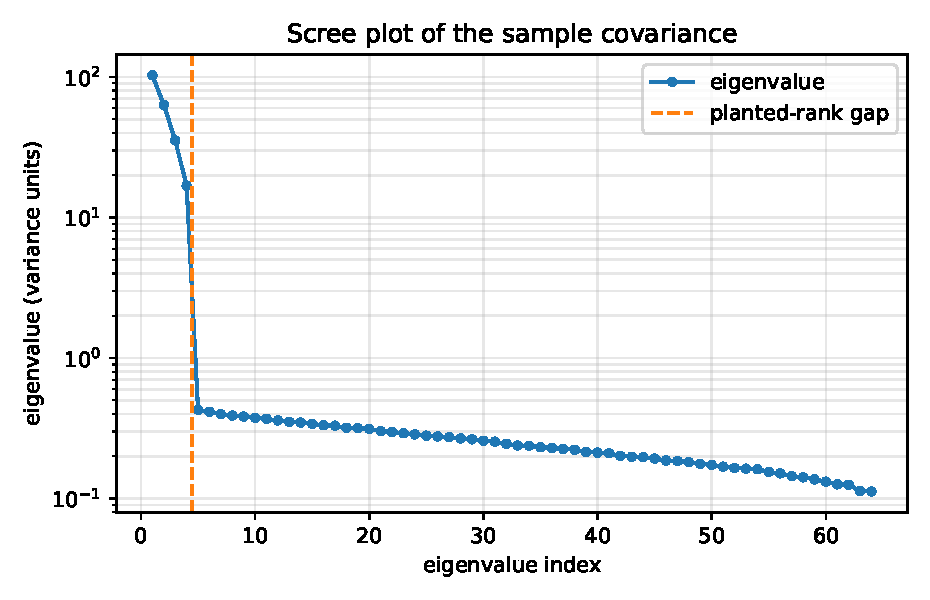
\includegraphics[width=0.82\textwidth]{scree.pdf}
\caption{Scree plot of \(\mat{C}\) (log \(y\)-axis). The dashed line sits
in the gap between the planted rank-\(4\) spectrum and the noise floor.}
\end{figure}

\begin{figure}[ht]
\centering
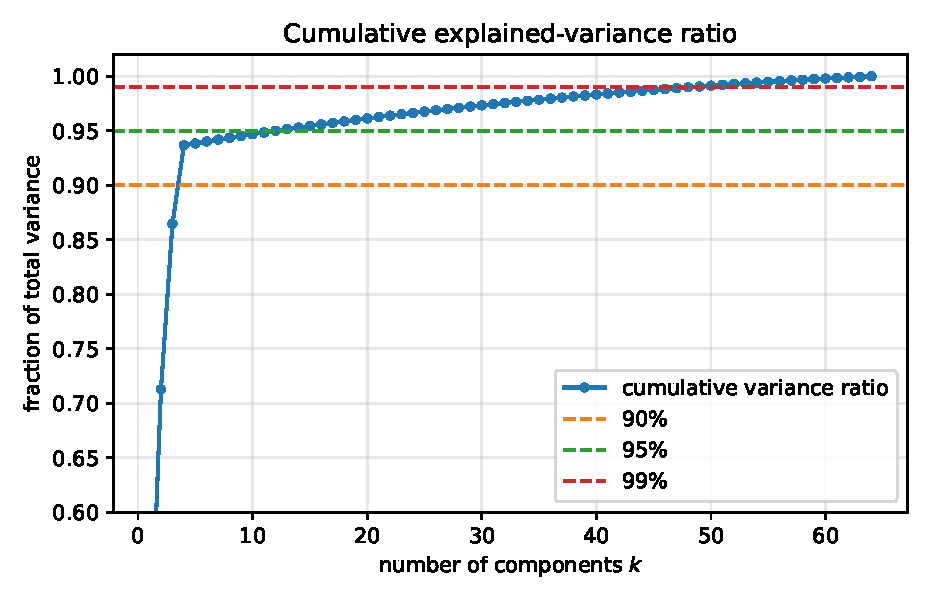
\includegraphics[width=0.82\textwidth]{cumulative_variance.pdf}
\caption{Cumulative explained-variance ratio. Horizontal lines are the
\(90\%\), \(95\%\), and \(99\%\) thresholds.}
\end{figure}

\paragraph{(i)}
Smallest \(k\) that retains at least that fraction of total variance:
\begin{center}
\begin{tabular}{cc}
    \toprule
    threshold & smallest \(k\) \\
    \midrule
    \(\ge 90\%\) & \(4\) \\
    \(\ge 95\%\) & \(13\) \\
    \(\ge 99\%\) & \(49\) \\
    \bottomrule
\end{tabular}
\end{center}
They disagree by a lot.

\paragraph{(ii)}
The scree plot has a clear order-of-magnitude cliff after index \(4\):
\[
\lambda_4 = 16.790, \qquad \lambda_5 = 0.428,
\qquad \lambda_4/\lambda_5 \approx 39.2.
\]

\paragraph{(iii)}
Only the \(90\%\) cutoff recovers \(r=4\). At \(k=4\) I already have
\(93.7\%\) of the variance, so \(90\%\) stops there. Everything after the
gap is noise, but that noise still adds up: \(64-4=60\) tiny eigenvalues
can be \(\sim 6\%\) of the trace, so \(95\%\) keeps grabbing noise
components until \(k=13\), and \(99\%\) keeps going to \(k=49\). Those two
are not selecting signal. They are just vacuuming the noise floor until
the leftover energy is small enough.

I would trust the spectral gap to size a compression scheme, not a fixed
variance threshold. The gap is telling you where the planted (or actual)
rank is. A \(95\%\) or \(99\%\) rule will happily spend SRAM on noise.

\paragraph{(iv)}
Prediction before rerunning: drop the noise std from \(0.5\) to \(0.05\)
and the noise variance falls by \(100\times\). The noise-floor trace is
then tiny next to \(10^2+8^2+6^2+4^2=216\). The first three planted
components are already about \(200/216\approx 93\%\), so I expected
\(90\%\) to move to \(k=3\), and both \(95\%\) and \(99\%\) to snap to
\(k=4\).

Rerun (same seed, \(\sigma=0.05\)): \(k_{90}=3\), \(k_{95}=4\),
\(k_{99}=4\), and \(\lambda_4/\lambda_5\approx 3838\). The prediction held.
The gap got huge, and a fixed \(90\%\) cutoff now undershoots the planted
rank instead of matching it. Another reason not to size \(k\) from a
variance percentage.

%----------------------------------------------------------------------
\subsection*{(d) Projection}

\begin{figure}[ht]
\centering
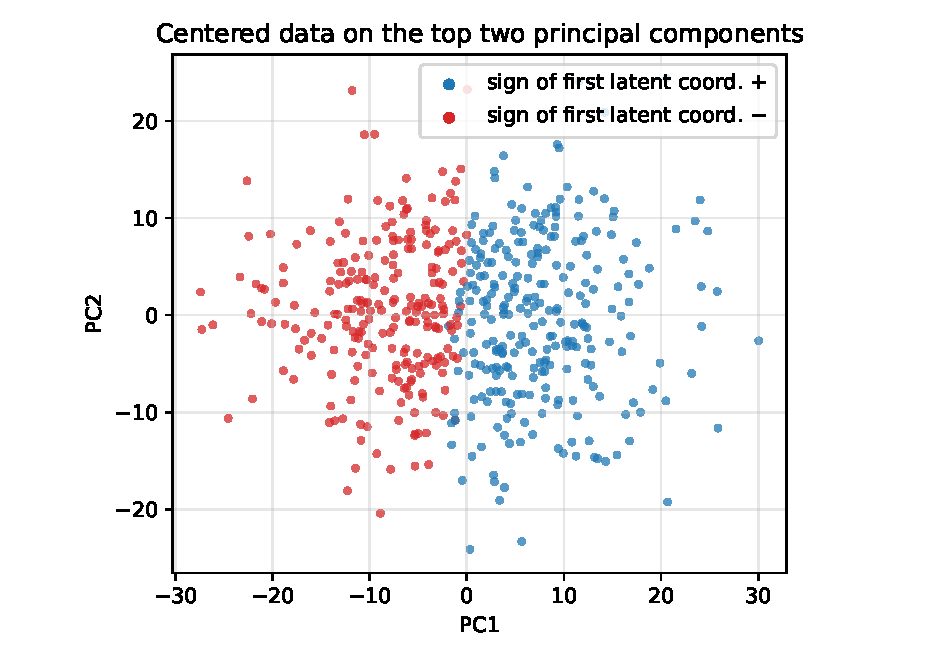
\includegraphics[width=0.82\textwidth]{pca_scatter.pdf}
\caption{Centered activations projected onto PC1 and PC2, colored by the
sign of the first column of the planted latent matrix \(\mat{Z}\).}
\end{figure}

PCA rotated the coordinates onto the directions of highest variance. PC1
lines up with the strongest planted factor (the \(D_{11}=10\) column of
\(\mat{Z}\)), so coloring by \(\mathrm{sign}(Z_{\cdot 1})\) splits the
cloud left/right. PC2 picks up the next factor, which is why the cloud is
spread on both axes and not just a 1-D line. If I had left the data
uncentered, the per-feature offset would have been a huge DC component
and PC1 would have pointed at that mean, not at the latent. The two
colors would sit on top of each other along a mean-dominated axis and the
plot would not show the planted structure.

%----------------------------------------------------------------------
\subsection*{(e) Reconstruction vs.\ the theoretical bound}

\begin{figure}[ht]
\centering
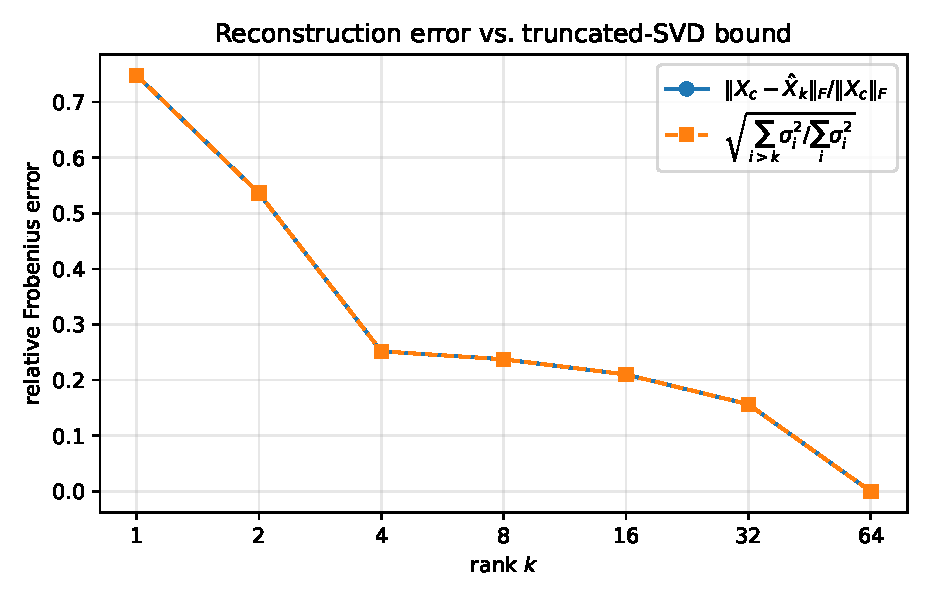
\includegraphics[width=0.82\textwidth]{reconstruction_error.pdf}
\caption{Relative Frobenius reconstruction error versus \(k\), with the
Eckart--Young--Mirsky curve overlaid. The two series sit on top of each
other.}
\end{figure}

The Eckart--Young--Mirsky theorem says the truncated SVD is the optimal
rank-\(k\) approximation in Frobenius norm, and
\[
\|\mat{X}_c-\hat{\mat{X}}_k\|_F
= \sqrt{\sum_{i>k}\sigma_i^2},
\]
so the two curves we were asked to plot have to coincide. Empirically the
maximum absolute gap is \(1.30\times 10^{-15}\) (just floating-point
noise; at \(k=64\) the leftover singular values are empty).

%----------------------------------------------------------------------
\subsection*{(f) The hardware payoff}

\paragraph{(i)}
Dense \(\mat{X}_c\) in FP32:
\[
M\cdot N\cdot 4\ \mathrm{B}
= 500\cdot 64\cdot 4
= 128000\ \mathrm{B}
= 125\ \mathrm{KB}.
\]

\paragraph{(ii)--(iii)}
Compressed form \(\{\mat{X}_c\mat{V}_k,\ \mat{V}_k\}\) costs
\((Mk+Nk)\cdot 4\) bytes. Compression ratio is
\(MN\big/\bigl(k(M+N)\bigr)\). Break-even when that ratio drops to \(1\):
\[
k(M+N) < MN \qquad\Rightarrow\qquad k < \frac{MN}{M+N} = \frac{32000}{564}
\approx 56.74.
\]
So the compressed form stops being a win once \(k\ge 57\). On the requested
grid that is \(k=64\) (ratio \(0.887\), \(141\ \mathrm{KB} > 125\ \mathrm{KB}\)).
At \(k=32\) it is still a \(1.77\times\) save.

\begin{center}
\begin{tabular}{crrrr}
    \toprule
    \(k\) & var.\ retained & footprint (KB) & ratio & proj.\ (\(\mu\)s) \\
    \midrule
    1  & \(0.441\) & \(2.20\)  & \(56.74\) & \(4.5\) \\
    2  & \(0.713\) & \(4.41\)  & \(28.37\) & \(11.2\) \\
    4  & \(0.937\) & \(8.81\)  & \(14.18\) & \(11.4\) \\
    8  & \(0.944\) & \(17.63\) & \(7.09\)  & \(16.5\) \\
    16 & \(0.956\) & \(35.25\) & \(3.55\)  & \(26.1\) \\
    32 & \(0.975\) & \(70.50\) & \(1.77\)  & \(49.2\) \\
    64 & \(1.000\) & \(141.00\)& \(0.89\)  & \(63.5\) \\
    \bottomrule
\end{tabular}
\end{center}

\paragraph{(iv)}
I timed only the projection \(\mat{X}_c\mat{V}_k\) on this CPU. For the
useful rank \(k=4\) it is about \(11\,\mu\mathrm{s}\) on a \(500\times 64\)
matrix, which is nothing. The point from lecture is still the one that
matters: SVD-on-weights is free at inference because you do it once
offline. PCA-on-activations is in the live path --- a new \(\mat{X}\)
shows up every layer / every batch, you have to center it, and you have
to multiply by \(\mat{V}_k\). To make that viable on-chip you need a
small MAC array that can do an \(M\times N\times k\) GEMM without going
back to DRAM, plus SRAM that already holds \(\mat{V}_k\), and you
probably want it fused with the layer that produced \(\mat{X}\) so the
dense activation never gets written out in full. Without that, the
``compression'' just moves the bandwidth problem into a runtime matmul.

\newpage
\section{Problem 4: Training LeNet-5}

I built LeNet-5 from primitive layers (no model zoo). MNIST is padded by 2
pixels on each side \emph{before} normalization, then normalized with
mean \(0.1307\) and std \(0.3081\). A random \(90/10\) split of the 60k
training images at seed \(511\) is the validation set. Optimizer is SGD
+ momentum \(0.9\), \(\eta=0.01\), batch \(64\), 15 epochs. Device is
local CPU, 32 cores, PyTorch \(2.14.0+cpu\). Code is
\texttt{problem4.py}.

I checked one padded tensor: the border value matches the background
(both become \((0-0.1307)/0.3081\approx -0.424\) after normalize), so
there is no mid-gray frame.

%----------------------------------------------------------------------
\subsection*{(a) Implementation and static analysis}

Output size \(H_{\mathrm{out}}=\lfloor(H_{\mathrm{in}}+2P-K)/S\rfloor+1\).
Conv: \(\#\mathrm{params}=C_{\mathrm{out}}(C_{\mathrm{in}}K^2+1)\),
\(\#\mathrm{MACs}=H_{\mathrm{out}}W_{\mathrm{out}}C_{\mathrm{out}}C_{\mathrm{in}}K^2\).
FC: \(\#\mathrm{params}=C_{\mathrm{out}}(C_{\mathrm{in}}+1)\),
\(\#\mathrm{MACs}=C_{\mathrm{out}}C_{\mathrm{in}}\).
Pooling is 0 params and 0 MACs; its activation traffic still counts in
bytes moved. Bytes moved = FP32 weights + input activations + output
activations (no reuse). Intensity \(=2\times\#\mathrm{MACs}/\)bytes.

\begin{center}
\footnotesize
\begin{tabular}{lccccc}
    \toprule
    Layer & Output & \#Params & \#MACs & Bytes moved & Intensity \\
    \midrule
    C1  & \(6\times28\times28\)   & \(156\)    & \(117{,}600\) & \(23{,}536\)  & \(9.99\) \\
    S2  & \(6\times14\times14\)   & \(0\)      & \(0\)         & \(23{,}520\)  & \(0\) \\
    C3  & \(16\times10\times10\)  & \(2{,}416\)& \(240{,}000\) & \(20{,}768\)  & \(23.11\) \\
    S4  & \(16\times5\times5\)    & \(0\)      & \(0\)         & \(8{,}000\)   & \(0\) \\
    C5  & \(120\times1\times1\)   & \(48{,}120\)& \(48{,}000\) & \(194{,}560\) & \(0.49\) \\
    F6  & \(84\)                  & \(10{,}164\)& \(10{,}080\) & \(41{,}472\)  & \(0.49\) \\
    Out & \(10\)                  & \(850\)    & \(840\)       & \(3{,}776\)   & \(0.44\) \\
    \midrule
    Total & n/a & \(61{,}706\) & \(416{,}520\) & \(315{,}632\) & \(2.64\) \\
    \bottomrule
\end{tabular}
\end{center}

Hand calc for C1: \(H_{\mathrm{out}}=(32-5)+1=28\),
params \(=6(25+1)=156\), MACs \(=28\cdot28\cdot6\cdot1\cdot25=117600\),
bytes \(=156\cdot4 + 32\cdot32\cdot4 + 6\cdot28\cdot28\cdot4=23536\),
intensity \(=235200/23536=9.99\).
C3: params \(=16(150+1)=2416\), MACs \(=10\cdot10\cdot16\cdot6\cdot25=240000\).
C5: params \(=120(400+1)=48120\), MACs \(=120\cdot16\cdot25=48000\).
F6: \(84\cdot121=10164\), Out: \(10\cdot85=850\).

PyTorch \texttt{numel()} on the same model: C1 \(156\), C3 \(2416\),
C5 \(48120\), F6 \(10164\), Out \(850\), total \(61706\). Matches the
hand table exactly. No mismatch to reconcile.

%----------------------------------------------------------------------
\subsection*{(b) Training}

\begin{center}
\footnotesize
\begin{tabular}{crrrrr}
    \toprule
    ep & train loss & train acc & val loss & val acc & time (s) \\
    \midrule
    1  & 0.434 & 0.8805 & 0.154 & 0.9538 & 27.6 \\
    2  & 0.104 & 0.9690 & 0.086 & 0.9730 & 13.7 \\
    3  & 0.067 & 0.9796 & 0.068 & 0.9778 & 14.0 \\
    4  & 0.052 & 0.9845 & 0.058 & 0.9825 & 14.4 \\
    5  & 0.043 & 0.9875 & 0.054 & 0.9835 & 14.8 \\
    6  & 0.036 & 0.9892 & 0.053 & 0.9815 & 15.2 \\
    7  & 0.031 & 0.9908 & 0.041 & 0.9870 & 14.9 \\
    8  & 0.028 & 0.9912 & 0.049 & 0.9840 & 15.0 \\
    9  & 0.024 & 0.9928 & 0.040 & 0.9877 & 14.8 \\
    10 & 0.021 & 0.9934 & 0.045 & 0.9863 & 15.2 \\
    11 & 0.019 & 0.9946 & 0.042 & 0.9872 & 15.4 \\
    12 & 0.017 & 0.9947 & 0.038 & 0.9888 & 16.0 \\
    13 & 0.016 & 0.9953 & 0.037 & 0.9870 & 34.0 \\
    14 & 0.013 & 0.9966 & 0.040 & 0.9878 & 34.4 \\
    15 & 0.013 & 0.9966 & 0.044 & 0.9860 & 33.7 \\
    \bottomrule
\end{tabular}
\end{center}

\begin{figure}[ht]
\centering
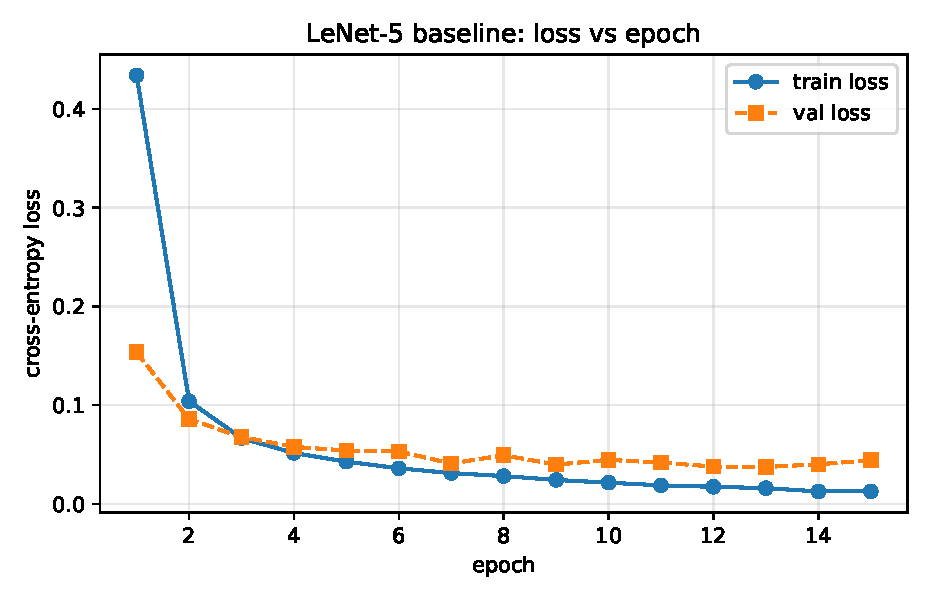
\includegraphics[width=0.48\textwidth]{lenet_baseline_loss.pdf}
\hfill
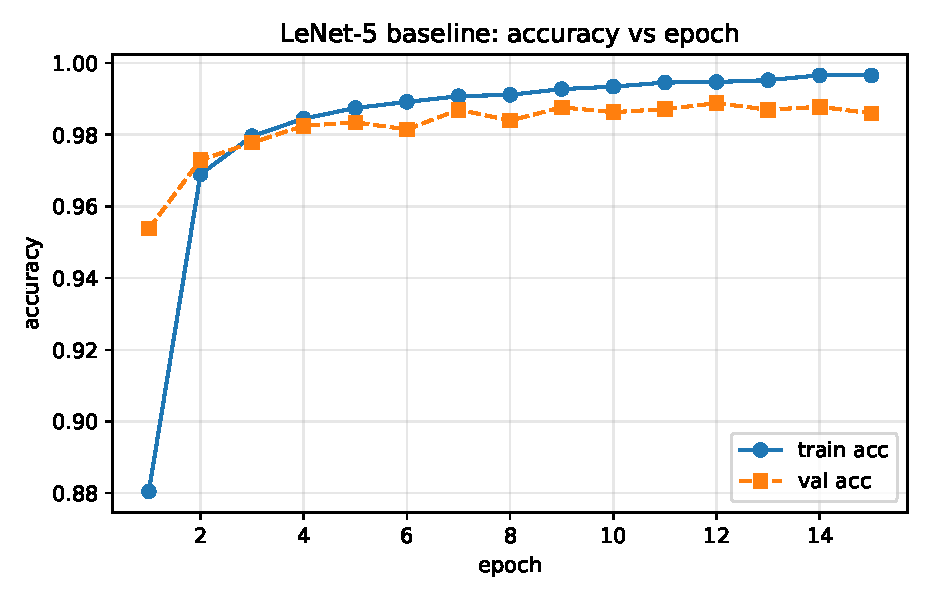
\includegraphics[width=0.48\textwidth]{lenet_baseline_acc.pdf}
\caption{Baseline LeNet-5 train/val loss and accuracy vs.\ epoch.}
\end{figure}

I would early-stop at epoch 12. That is the best validation accuracy
(\(0.9888\)). After that train accuracy keeps climbing and val accuracy
wobbles down a bit, so we are starting to overfit.

%----------------------------------------------------------------------
\subsection*{(c) Test-set evaluation}

Checkpoint from epoch 12. Test loss \(0.0287\), top-1 accuracy
\(0.9906\).

\begin{center}
\footnotesize
\begin{tabular}{crrr}
    \toprule
    class & precision & recall & F1 \\
    \midrule
    0 & 0.991 & 0.995 & 0.993 \\
    1 & 0.996 & 0.995 & 0.996 \\
    2 & 0.989 & 0.998 & 0.994 \\
    3 & 0.986 & 0.995 & 0.991 \\
    4 & 0.993 & 0.988 & 0.990 \\
    5 & 0.994 & 0.988 & 0.991 \\
    6 & 0.994 & 0.991 & 0.992 \\
    7 & 0.986 & 0.988 & 0.987 \\
    8 & 0.991 & 0.980 & 0.986 \\
    9 & 0.985 & 0.987 & 0.986 \\
    \bottomrule
\end{tabular}
\end{center}

\begin{figure}[ht]
\centering
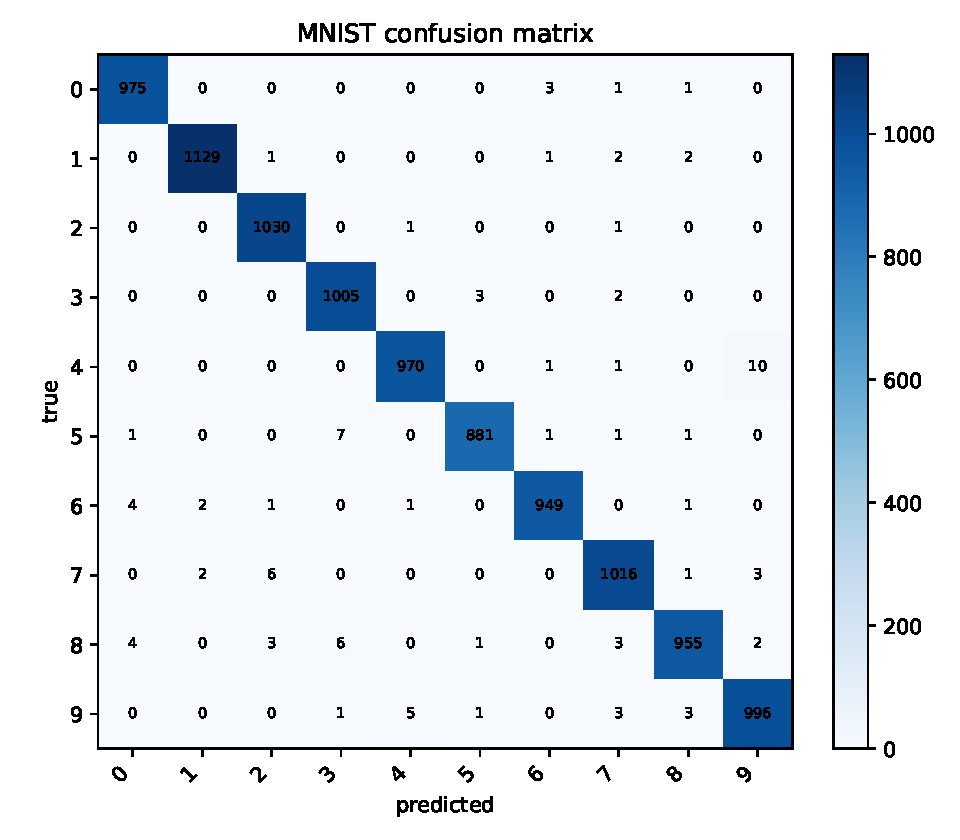
\includegraphics[width=0.72\textwidth]{cm_mnist.pdf}
\caption{MNIST \(10\times10\) confusion matrix for the baseline checkpoint.}
\end{figure}

\begin{figure}[ht]
\centering
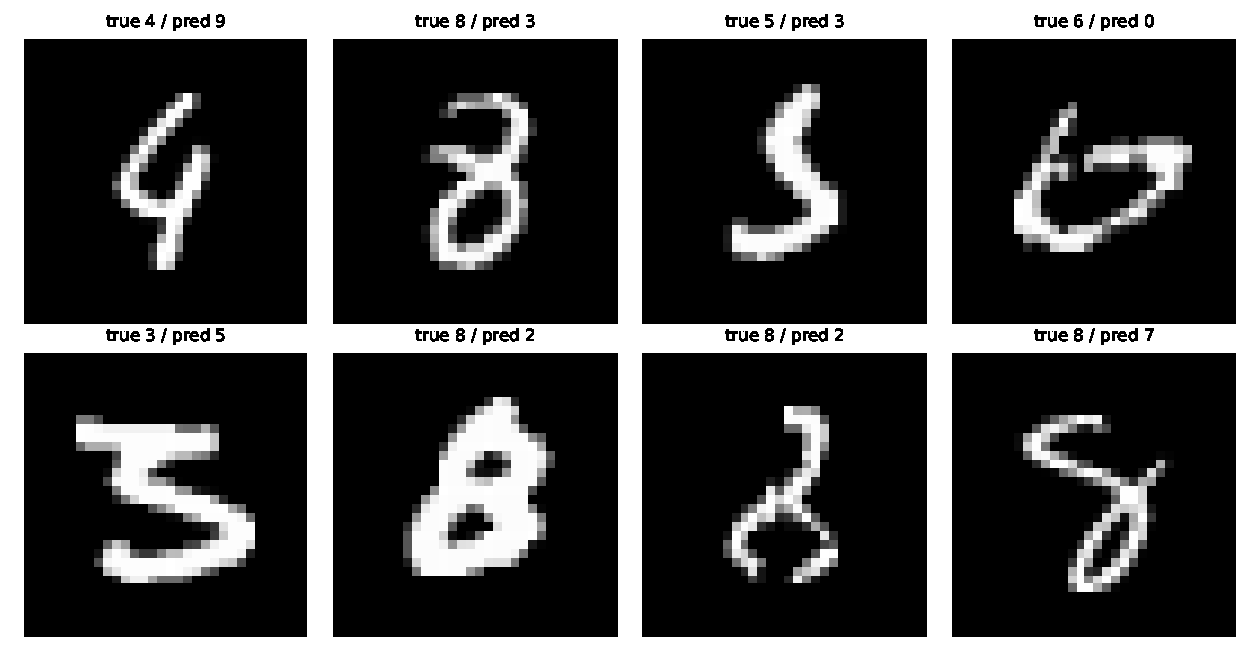
\includegraphics[width=0.92\textwidth]{misclassified_mnist.pdf}
\caption{Eight misclassified MNIST test images with true / predicted labels.}
\end{figure}

The two most-confused pairs are \(4\leftrightarrow 9\) (\(10+5=15\)
off-diagonal) and \(3\leftrightarrow 5\) (\(7+3=10\)). Those digits really
do look alike: a closed 4 is a 9 without the tail, and 3 vs.\ 5 is mostly
whether the top-left stroke connects. A 32-pixel grayscale net with no
augmentation is going to mix those.

%----------------------------------------------------------------------
\subsection*{(d) Ablations}

I ran four of the list (activation, pooling, learning rate, batch size),
one factor at a time from the baseline. ``Noise'' is the standard
deviation of the baseline test accuracy across seeds \(511,512,513\):
mean \(0.9896\), \(\mathrm{sd}=0.00090\) (about \(0.09\) points). I treat
gaps under \(\sim 0.3\) points as within noise.

\begin{center}
\footnotesize
\begin{tabular}{lccc}
    \toprule
    config & test acc & best val acc & mean epoch (s) \\
    \midrule
    baseline (tanh, avg, \(0.01\), \(64\)) & \(0.9906\) & \(0.9888\) & \(19.5\) \\
    ReLU & \(0.9903\) & \(0.9887\) & \(31.9\) \\
    max-pool & \(0.9907\) & \(0.9882\) & \(24.7\) \\
    lr \(0.1\) & \(0.9884\) & \(0.9863\) & \(16.6\) \\
    lr \(0.001\) & \(0.9765\) & \(0.9715\) & \(16.7\) \\
    batch \(16\) & \(0.9907\) & \(0.9905\) & \(25.7\) \\
    batch \(256\) & \(0.9858\) & \(0.9825\) & \(15.0\) \\
    \bottomrule
\end{tabular}
\end{center}

ReLU vs.\ tanh is within seed noise; on this tiny net it does not matter.
Avg-pool vs.\ max-pool is also within noise. lr \(0.1\) is a little
noisier / slightly worse; lr \(0.001\) is clearly too small and is still
climbing at epoch 15. Batch \(16\) has the best validation accuracy
(more steps per epoch); batch \(256\) is faster but underfits a bit in
15 epochs because there are fewer updates.

%----------------------------------------------------------------------
\subsection*{(e) Transfer to Fashion-MNIST}

Best config by validation accuracy was batch \(16\) (same everything
else). I retrained that on Fashion-MNIST with mean \(0.286\), std
\(0.353\). For the record, MNIST used \(0.1307\) / \(0.3081\).

Test accuracy \(0.8958\), test loss \(0.323\).

\begin{center}
\footnotesize
\begin{tabular}{lrrr}
    \toprule
    class & precision & recall & F1 \\
    \midrule
    T-shirt/top & 0.843 & 0.857 & 0.850 \\
    Trouser     & 0.991 & 0.963 & 0.977 \\
    Pullover    & 0.827 & 0.852 & 0.839 \\
    Dress       & 0.846 & 0.943 & 0.892 \\
    Coat        & 0.858 & 0.801 & 0.828 \\
    Sandal      & 0.976 & 0.967 & 0.971 \\
    Shirt       & 0.761 & 0.691 & 0.724 \\
    Sneaker     & 0.919 & 0.977 & 0.947 \\
    Bag         & 0.959 & 0.979 & 0.969 \\
    Ankle boot  & 0.978 & 0.928 & 0.952 \\
    \bottomrule
\end{tabular}
\end{center}

\begin{figure}[ht]
\centering
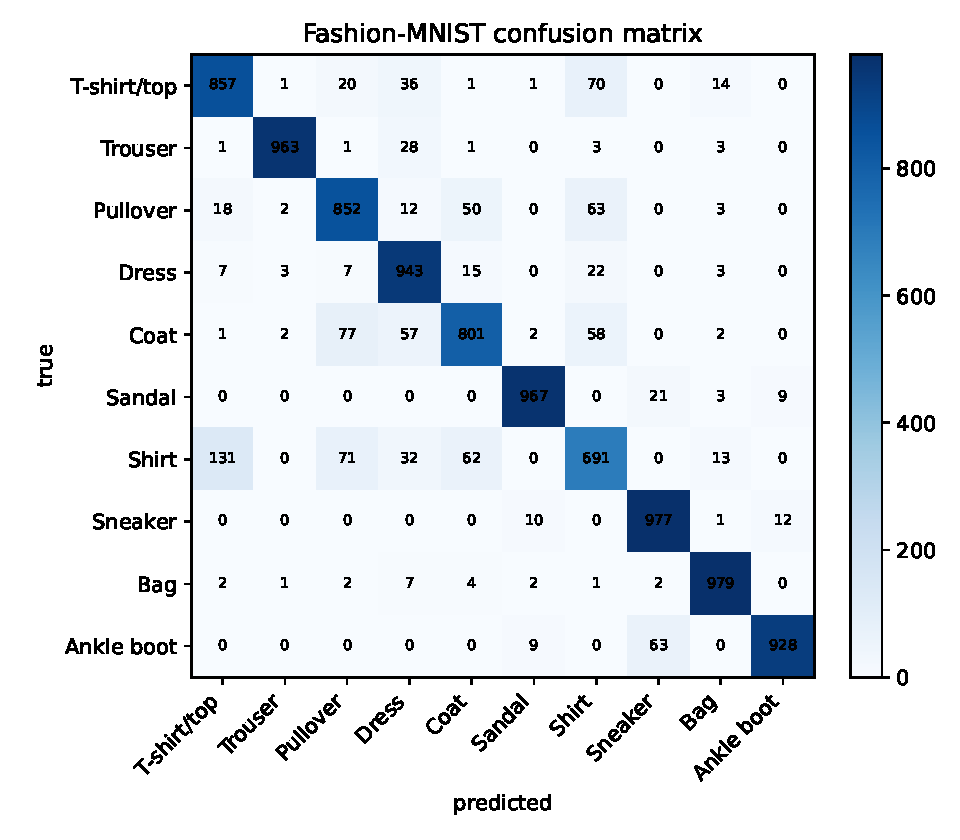
\includegraphics[width=0.78\textwidth]{cm_fashion.pdf}
\caption{Fashion-MNIST confusion matrix (best MNIST config, batch \(16\)).}
\end{figure}

The MNIST \(\to\) Fashion gap is about \(9.5\) points (\(0.9906\) vs.\
\(0.8958\)). Both: the task is harder, and the net is a bit
under-capacity. Evidence from my runs: on MNIST, train vs.\ val at the
chosen epoch is \(0.995\) vs.\ \(0.989\) (half a point). On Fashion it is
\(0.939\) vs.\ \(0.905\) (about \(3.4\) points), so we already overfit
more. Per-class, Shirt is a mess (F1 \(0.72\)) and it bleeds into
T-shirt, Pullover, and Coat --- those garments actually look alike,
unlike digits.

%----------------------------------------------------------------------
\subsection*{(f) Where the compute is, and where the parameters are}

I am answering (f) from the (a) table, before the training discussion.

\paragraph{(i)}
MACs are dominated by C3 (\(240{,}000\)) then C1 (\(117{,}600\)).
Parameters are dominated by C5 (\(48{,}120\)) then F6 (\(10{,}164\)).
Early convs slide a tiny filter over a big map, so you get a lot of MACs
from few weights. C5 is a \(5\times5\) conv that exactly covers its
input, i.e.\ a dense \(400\to120\) multiply, so the weight matrix is
large and each weight is used once. Same story for F6/Out.

\paragraph{(ii)}
Machine balance \(I_{\mathrm{balance}}=40\) FLOPs/byte. Every layer is
under that (max is C3 at \(23.1\)), so they are all memory-bound,
including the pools at intensity \(0\). That is not an arithmetic bug.
The no-reuse model charges the full weight tensor on every layer even
though a real accelerator would keep those weights in SRAM and amortize
them. With weights treated as streaming traffic, intensity stays small.

\paragraph{(iii)}
At batch \(B\), weights are paid once and activations scale with \(B\):
\[
I(B)=\frac{2B\cdot\mathrm{MACs}_1}{W + B(A_{\mathrm{in}}+A_{\mathrm{out}})}.
\]
As \(B\to\infty\), \(I\to 2\,\mathrm{MACs}_1/(A_{\mathrm{in}}+A_{\mathrm{out}})\).

C1: that ceiling is \(235200/22912\approx 10.27<40\). The coefficient of
\(B\) in \(2M-40A\) is negative, so \emph{no} batch size pushes C1 past
\(40\).

C3: the ceiling is \(480000/11104\approx 43.23>40\). Solving
\(I(B)>40\) gives \(B>10.79\), so the smallest integer batch is
\(B=11\).

Batching is how you amortize the weight traffic. Even then C1 never
becomes compute-bound under this traffic model, which is why people also
care about on-chip reuse / weight-stationary dataflow, not just \(B\).

\paragraph{(iv)}
Model size (parameters only): FP32 is
\(61706\times4/10^6=0.247\,\mathrm{MB}\). INT8 is
\(61706\times1/10^6=0.062\,\mathrm{MB}\).
Quantization helps the parameter-heavy layers most (C5, then F6) because
that is where the bytes are. Weight-stationary dataflow helps the
high-reuse convs: C1 has \(117600/156\approx 754\) MACs per weight, C3
has \(\approx 99\). C5 is about \(1\) MAC/weight, so stationary weights
do almost nothing there.

%----------------------------------------------------------------------
\subsection*{(g) Post-hoc low-rank compression}

No retraining. I reshaped C5 to \(120\times400\) and F6 to \(84\times120\),
took truncated SVD, and put the rank-\(r\) factors back. \(r\) is clipped
per layer (\(r\le 84\) on F6).

\begin{center}
\begin{tabular}{crr}
    \toprule
    \(r\) & test acc & factored params (\(U_r\Sigma_r\), \(V_r^\top\)) \\
    \midrule
    1   & \(0.1932\) & \(724\) \\
    2   & \(0.3604\) & \(1{,}448\) \\
    4   & \(0.7409\) & \(2{,}896\) \\
    8   & \(0.9775\) & \(5{,}792\) \\
    16  & \(0.9882\) & \(11{,}584\) \\
    32  & \(0.9899\) & \(23{,}168\) \\
    64  & \(0.9906\) & \(46{,}336\) \\
    120 & \(0.9906\) & \(79{,}536\) \\
    \bottomrule
\end{tabular}
\end{center}

\begin{figure}[ht]
\centering
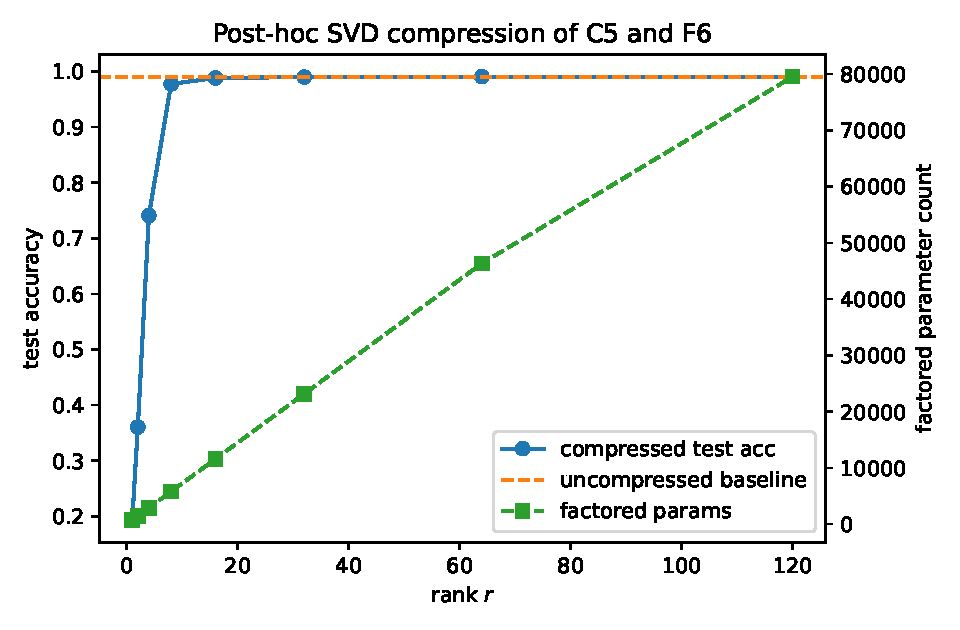
\includegraphics[width=0.82\textwidth]{svd_acc_vs_rank.pdf}
\caption{Test accuracy vs.\ rank after substituting truncated SVD into C5
and F6. Dashed line is the uncompressed baseline. Right axis is the
factored parameter count.}
\end{figure}

Smallest \(r\) within \(1\) absolute point of the \(0.9906\) baseline is
\(r=16\) (acc \(0.9882\)). \(r=8\) is \(0.9775\), which is more than a
point down. Those two layers had \(120\cdot400+84\cdot120=58080\)
weights; the factored form at \(r=16\) has \(11584\), so about an
\(80\%\) cut on just those two matrices.

Eckart--Young--Mirsky says this truncation is optimal in Frobenius norm.
LoRA writes \(y=W x + BA x\) with a frozen \(W\) and a trained low-rank
residual \(BA\). What I did is the same factorization idea
(\(U_r\Sigma_r\) plays the role of \(B\), \(V_r^\top\) of \(A\)), but I
\emph{replaced} the trained \(W\) instead of adding a residual, and I did
not train the factors.

\begin{figure}[ht]
\centering
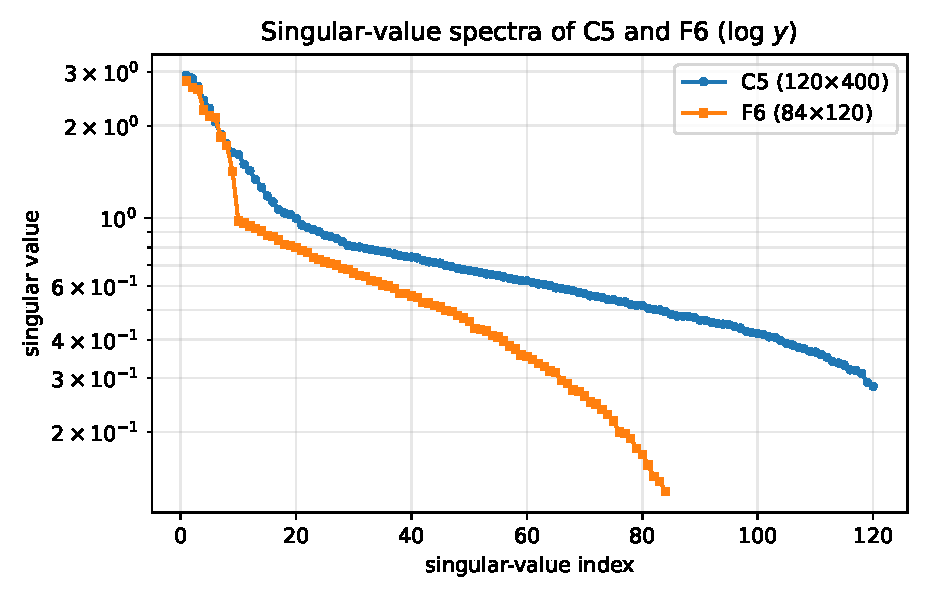
\includegraphics[width=0.82\textwidth]{svd_spectra.pdf}
\caption{Singular-value spectra of C5 and F6 on a log axis.}
\end{figure}

The accuracy cliff is between \(r=4\) and \(r=8\), then it is basically
flat after \(16\). The spectra decay smoothly --- there is no giant gap
at \(8\) --- so the cliff is a bit earlier than a visual knee. That still
says the trained weight matrices are redundant: you can throw away most
of the tail and the classifier barely notices.

\end{document}
